\chapter{Технологический раздел}
\label{cha:impl}

Необходимо выбрать и обосновать выбранный язык программирования и средства разработки.
Разработать эффективно работающую струтуру программы и протестировать программу.

\section{Выбор и обоснование языка программирования}

Для визуализации большого количества частиц в реальном времени необходимо высокая производительность
используемых инструментов, а также удобный способ распараллеливания на видеокарту для повышения
скорости отрисовки. Был выбан язык программирования C++ с фреймворком Qt, в котором реализованы классы
для взаимодействия с OpenGL и шейерами \cite{QtOpenGL}.

\section{Интерфейс пользователя}

Интерфейс представлен на рисунке \ref{img:interface}

\begin{figure}[H]
    \centering
    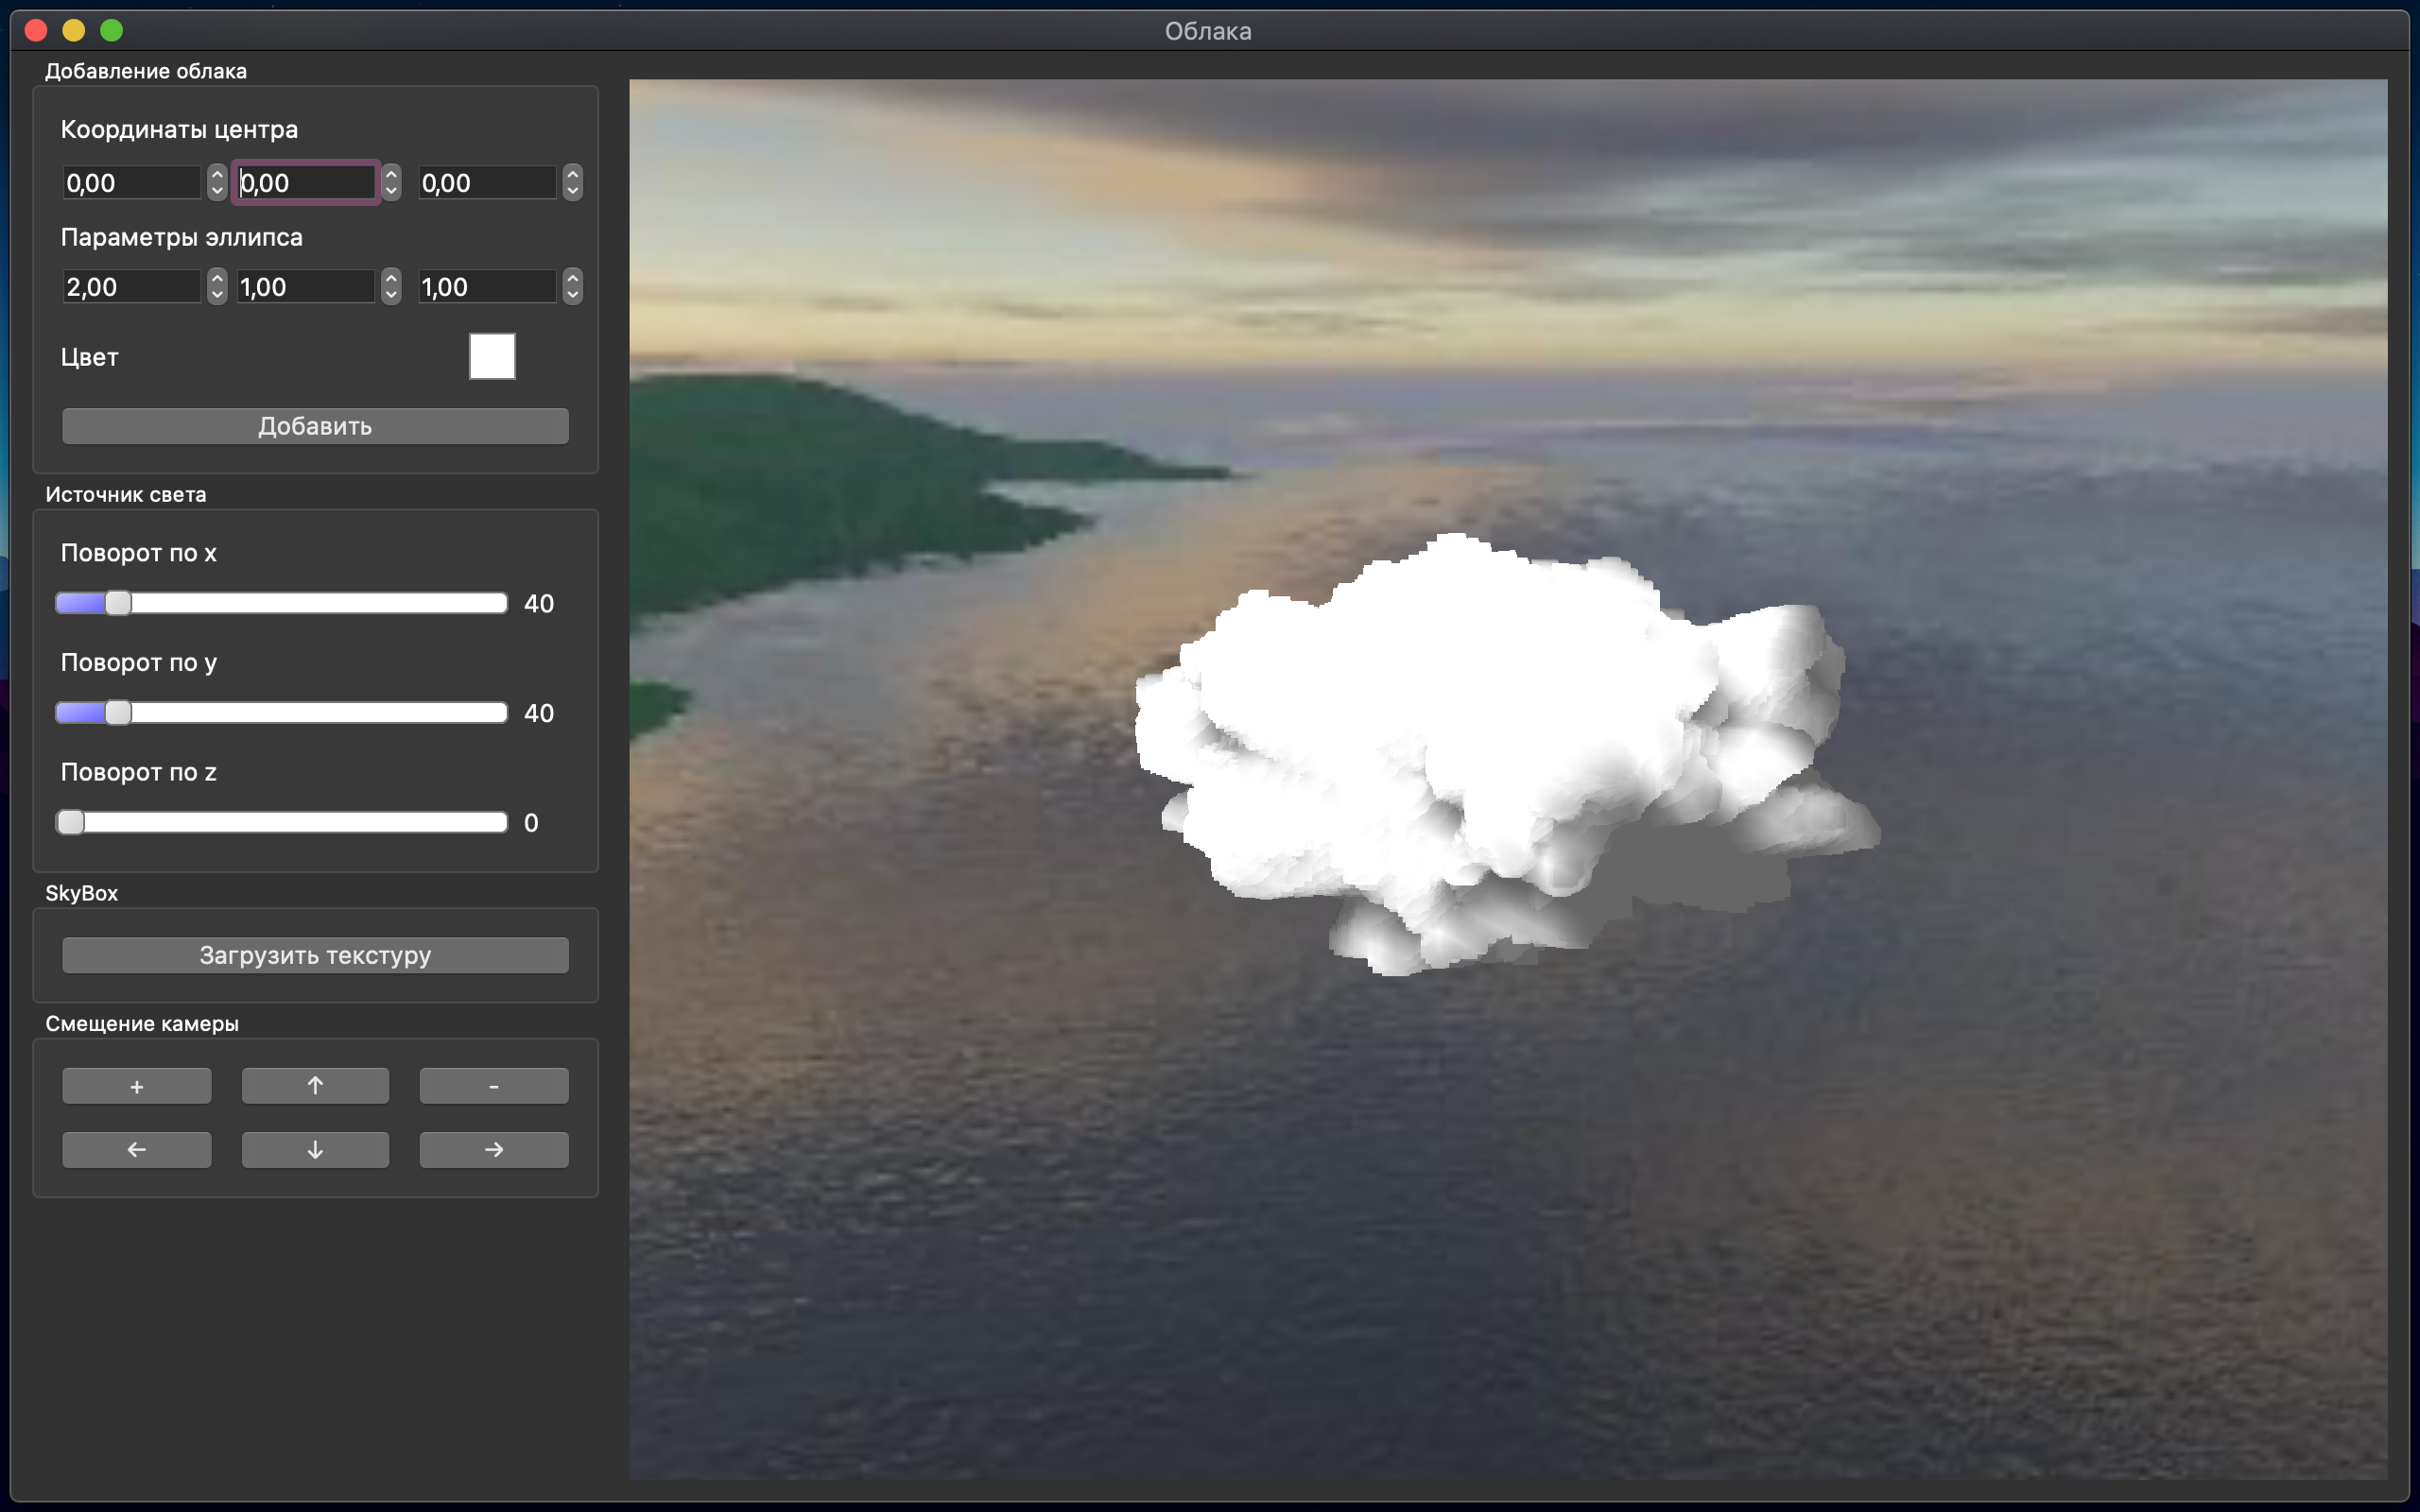
\includegraphics[scale=0.35]{img/interface.png}
    \caption{Интерфейс пользователя}
    \label{img:interface}
\end{figure}

Интерфейс позволяет добавлять облака с параметрами генерации, координатами центра и цветом.
Помимо этого имеется возможность вращать источник света вокруг центра системы координат с помощью ползунков.
Копки позволяют перемещать камеру по осям $x$ и $y$, а колесико мыши -- по $z$. Также с помощью мыши
можно вращать камеру вокруг центра координат.

\section{Хранение и обмен данными в системе}

Для хранения частиц используется класс частицы (таблица \ref{table:particle}).

\begin{table}[H]
    \centering
    \caption{Класс частицы}
    \label{table:particle}
    \begin{tabular}{|l|}
        \hline
        \multicolumn{1}{|c|}{\textbf{Particle}} \\
        \hline
        --\underline{arrayBuffer} : QOpenGLBuffer \\
        --\underline{indexBuffer} : QOpenGLBuffer \\
        --modelViewMatrix : QMatrix4x4 \\
        --r : float \\
        --g : float \\
        --b : float \\
        \hline
        +Particle( ) \\
        +Particle( x : float, y : float, z : float ) \\
        +Particle( x : float, y : float, z : float, r : float, g : float, b : float ) \\
        +\underline{initialization}( ) \\
        +\underline{firstDraw}( program : QOpenGLShaderProgram ) \\
        +draw( program : QOpenGLShaderProgram, functions : QOpenGLFunctions ) \\
        +setColor( r : float, g : float, b : float ) \\
        \hline
    \end{tabular}
\end{table}

\section{ER-модель}

При разработке приложения использован объекто-ориентированный подход. Модель классов
видно на рисунке \ref{img:er}

\begin{figure}[H]
    \centering
    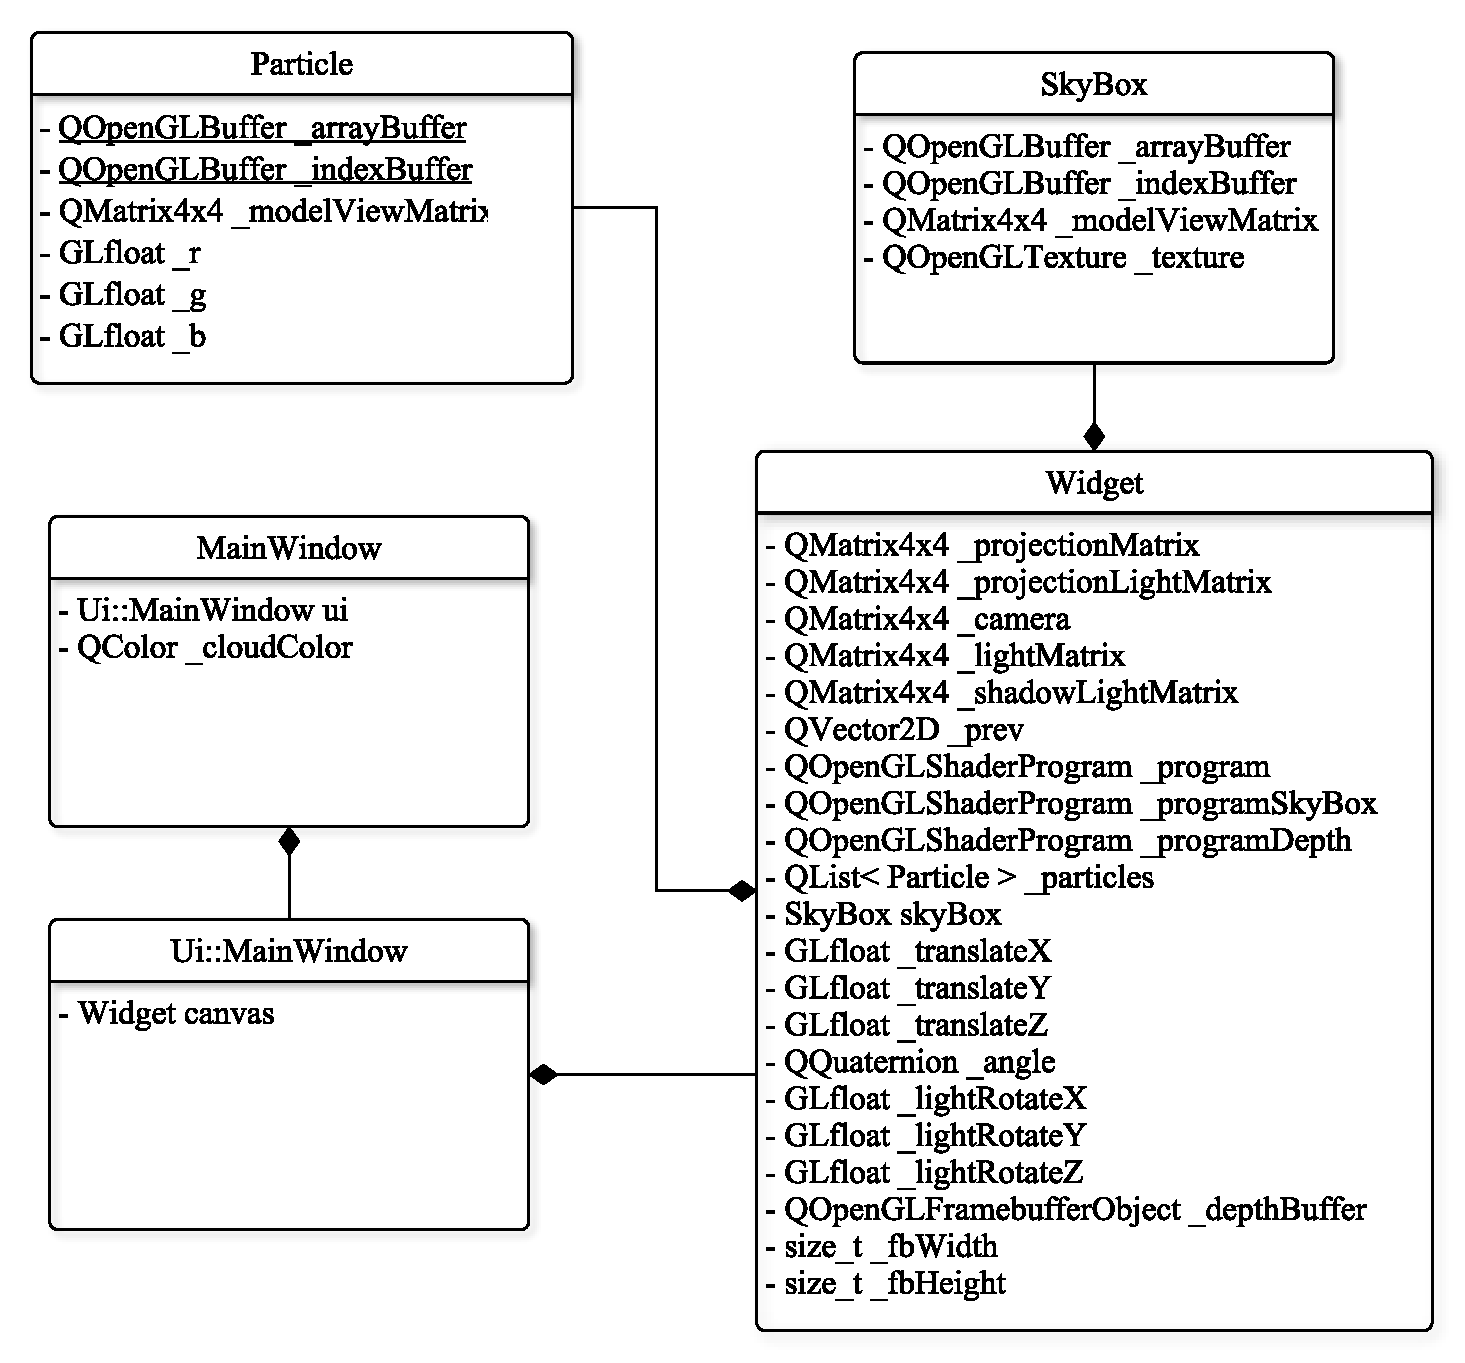
\includegraphics[scale=0.6]{img/er.pdf}
    \caption{ER-модель классов}
    \label{img:er}
\end{figure}

\section{Требования к аппаратуре}

Если необходимо визуализировать много облаков, требуется дискретная
видеокарта для комфортной частоты кадров.

\section{Тестирование}

Было проведено функциональное тестирование белого ящика, в ходе которого программа отработала
правильно. Также проведено тестирование пользовательского интерфейса, все элементы
интерфейса реагируют корректно.

\section{Выводы}

Был реализован алгоритм на выбранном языке C++. Программа полностью прошла функциональное тестирование
и тестирование интерфейса.

%%%% mode: latex
%%%% TeX-master: "rpz"
%%%% End:
